\newpage
\section{Attività di analisi requisiti utente}
\subsection{Resoconto delle attività di verifica}

Dopo aver redatto tutti i documenti presenti nella Revisione dei Requisiti, il team ha svolto le attività di verifica su di essi e sui processi analizzati. I documenti sono stati sottoposti al processo di analisi statica definito nel documento \NdP{}.
Prima è stata utilizzata la tecnica del Walkthrough, segnalando gli errori incontrati tramite una lettura approfondita in un'apposita lista presa in carico dal Verificatore per attuare la correzione del documento. In seguito la stessa lista è stata utilizzata per la tecnica dell'Inspection, che è servita ad individuare la presenza di nuovi errori utilizzando il confronto della lista di quelli commessi in precedenza.
In seguito i documenti sono stati interamente verificati secondo le metriche descritte nell'Appendice~\nameref{AppB:metric}, e sono stati riportati i risultati ottenuti.

\subsection{Verifica dei processi}
\subsubsection{Schedule Variance}
Nel seguente grafico vengono riportati i valori ottenuti calcolando la Schedule Variance sui tempi di stesura di ogni documento rispetto ai tempi prefissati nel \PdP{}:

\begin{figure}[h!]
	\centering
	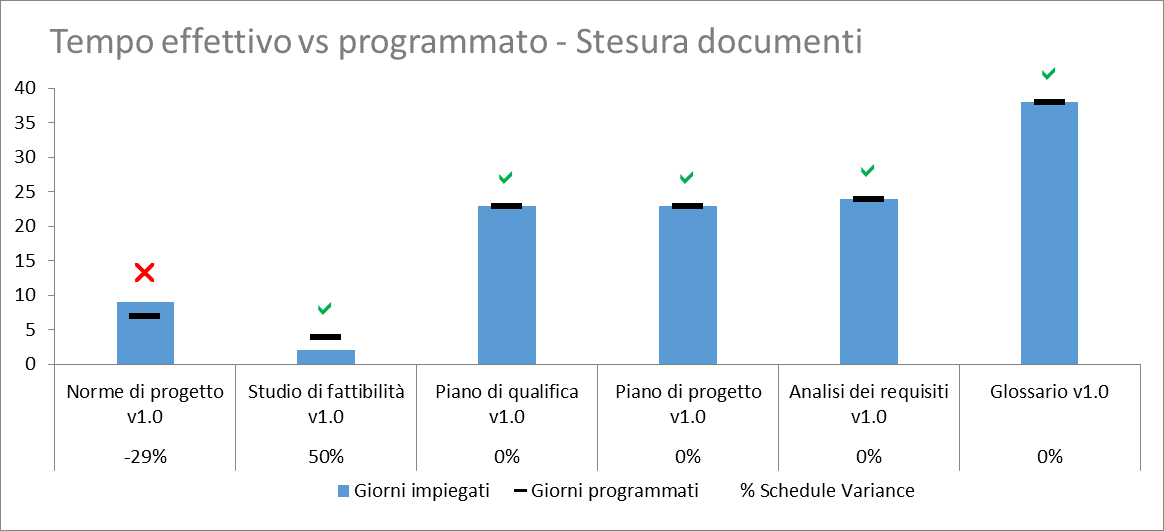
\includegraphics[scale=0.75]{img/Grafici/SV-Documenti.png}
		\caption{Schedule Variance per la stesura di ogni documento; \textcolor{green}{\checkmark} indica il raggiungimento della soglia di ottimalità, mentre \textcolor{red}{x} indica il non raggiungimento della soglia di accettabilità.}
	\label{fig:SV-Documenti}
\end{figure}

\begin{itemize}
	\item Schedule Variance finale: 0. 
	Il grafico evidenzia uno sforamento dei tempi riservati alla stesura delle \emph{Norme di Progetto}, il quale viene però compensato da un anticipo sui tempi di stesura dello \emph{Studio di fattibilità}: il ritardo si quantifica in 2 giorni, esattamente come l'anticipo, mentre per la stesura degli altri documenti si sono rispettati i tempi previsti. 
	
	\item Soglia raggiunta: ottimalità.
\end{itemize}

\subsubsection{Cost Variance}
Il calcolo della Cost Variance sul \emph{processo di documentazione} ha portato il seguente risultato: 

{
\renewcommand{\arraystretch}{2}
\centering
\begin{tabular}{| c | c | c | c | c |}
	\hline
	\textbf{Processo} & \textbf{BCWP} & \textbf{ACWP} & \textbf{CV} & \textbf{Valutazione} \\
	\hline
	Verifica & 3870\euro & 3840\euro & 0,78\% & Ottimale \\
	\hline
\end{tabular}

}


\subsection{Verifica dei documenti}
\subsubsection{Schedule Variance}
Nels seguente grafico vengono riportati i valori ottenuti calcolando la Schedule Variance sui tempi di verifica di ogni documento rispetto ai tempi prefissati nel'\textit{Piano di Progetto}:

\begin{figure}[h!]
	\centering
	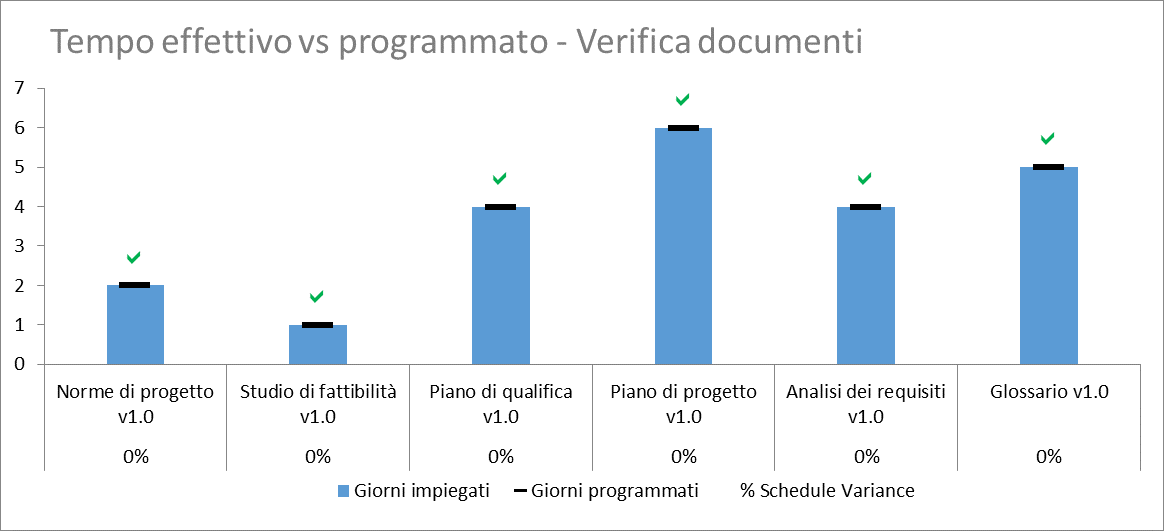
\includegraphics[scale=0.75]{img/Grafici/SV-VerDocumenti.png}
	\caption{Schedule Variance per la verifica di ogni documento; \textcolor{green}{\checkmark} indica il raggiungimento della soglia di ottimalità, mentre \textcolor{red}{x} indica il non raggiungimento della soglia di accettabilità.}
	\label{fig:SV-VerDocumenti}
\end{figure}

\begin{itemize}
	\item Schedule Variance finale: 0. 
	Il processo di verifica è stato completato senza anticipi nè ritardi.
	
	\item Soglia raggiunta: ottimalità.
\end{itemize}


\subsubsection{Cost Variance}
Il calcolo della Cost Variance sul \emph{processo di verifica} ha portato il seguente risultato: 

{
	\renewcommand{\arraystretch}{2}
	\centering
	\begin{tabular}{| c | c | c | c | c |}
		\hline
		\textbf{Processo} & \textbf{BCWP} & \textbf{ACWP} & \textbf{CV} & \textbf{Valutazione} \\
		\hline
		Verifica & 300\euro & 300\euro & 0\% & Ottimale \\
		\hline
	\end{tabular}

}

\subsubsection{Errori ortografici}
Sono stati rilevati errori ortografici all'interno dei documenti analizzati secondo i seguenti parametri:
{
	\renewcommand{\arraystretch}{2}
	\centering
	\begin{tabular}{| c | C{1cm} | C{3cm} |}
			\hline
		Analisi dei Requisiti v1.0 & 1\% & Accettabile \\
			\hline
		Norme di Progetto v1.0 & 2\% & Accettabile\\
			\hline
		Studio di Fattibilità v1.0 & 1\% &  Accettabile \\
			\hline
		Piano di Progetto v1.0 & 1\% & Accettabile \\
			\hline
		Piano di Qualifica v1.0 & 2\% & Accettabile\\
			\hline
		Glossario v1.0 & 1\% & Accettabile\\
			\hline
	\end{tabular}

}

Errori Ortografici calcolati: +2%.
Soglia raggiunta: accettabilità.


\subsubsection{Indice Gulpease}

Tutti i documenti consegnati sono stati sottoposti al calcolo dell'Indice Gulpease per valutarne il grado di leggibilità.
Sono stati rilevati i seguenti indici di leggibilità:

{
	\renewcommand{\arraystretch}{2}
	\centering
	\begin{tabular}{| c | C{3cm} | C{3cm} |}
			\hline
		Analisi dei Requisiti v1.0 &  mancanti & Accettabile \\
			\hline
		Norme di Progetto v1.0 & mancanti & Accettabile\\
			\hline
		Studio di Fattibilità v1.0 & mancanti & Accettabile\\ 
			\hline
		Piano di Progetto v1.0 & mancanti & Accettabile \\
			\hline
		Piano di Qualifica v1.0 & mancanti & Accettabile\\
			\hline
		Glossario v1.0 & mancanti & Accettabile\\
			\hline
	 \end{tabular}
 
}

Indice Gulpease:
Soglia raggiunta:

\subsubsection{Errori concettuali}

Nella seguente tabella vengono riportati i valori ottenuti calcolando la percentuale degli errori concettuali tramite la formula presente nell'appendice in sezione ~\nameref{AppB:ErroriCont}.

%Errori concettuali & 0\% & Ottimale   

Errori concettuali calcolati:
Soglia raggiunta:
